\chapter{基于辐射度量学的光线追踪}

Whitted sytle ray tracing并不能精确地给到正确的结果,精准给光物理量的方法。

\section{Radiant Energy and Flux(Power)}

\subsection*{辐射能量(radiant energy)}
在辐射度量学中,最基本的单位是\textsl{辐射能量},辐射能量$Q$是以辐射的形式发射、传播或者接收的能量。每个
光子都携带一定的能量,这个能量正比于频率$v$

\begin{equation}
    Q[J=Joule]=hv
\end{equation}

其中$h=6.62620\times 10^{-34}\ J\cdot s$为普朗克常数。

\subsection*{辐射流量(Radiant flux)}

辐射通量(radiant flux)记为 ,表示光源每秒钟发射的功率($dQ/dt$),
其单位为瓦特(watt)W ,例如一个灯泡可能发射 $100$ 瓦特的辐射通量。在辐
射测量中,都是基于这个辐射通量来测试能量,而不是使用总的能量 Q,所以
以下这些度量都是在单位时间(每秒)下发生的。

\begin{equation}
    \phi=\frac{dQ}{dt}\ \ [W=Watt][lm=lumen]
\end{equation}

\begin{figure}[H]
    \centering
    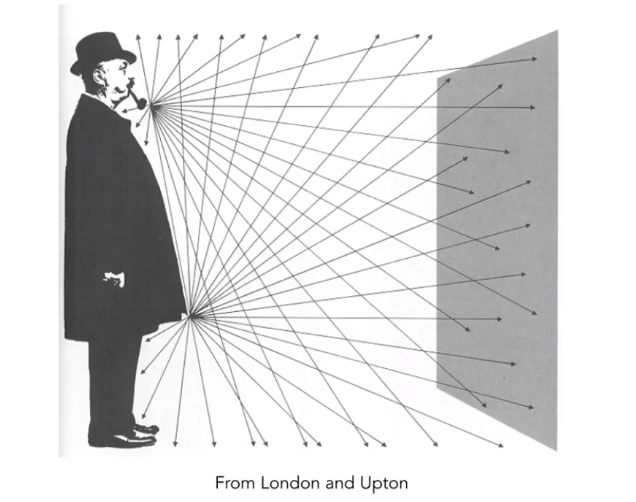
\includegraphics[scale=0.4]{figures/flux.png}
    \caption{flux}
\end{figure}

\section{立体角(soild angle)}

\subsection*{怎么去定义一个角度?}

用弧度定义一个角
\begin{equation}
    \theta=\frac{l}{r}
\end{equation}

立体角是三维空间中的延伸
\begin{equation}
    \Omega=\frac{A}{r^2}
\end{equation}

\subsection*{微分立体角}

整个球面上的立体角积分
\begin{equation}
    \Omega=\int_{S^2}d\omega=4\pi
\end{equation}

\begin{equation}
    dA=(rd\theta)(rsin\theta d\phi)=r^2sin\theta d\theta d\phi
\end{equation}

\begin{equation}
    d\omega=\frac{dA}{r^2}=sin\theta d\theta d\phi
\end{equation}

\subsection*{Isotropic Point Source}

\begin{equation}
    \phi=\int_{S^2}Id\omega=4\pi I
\end{equation}


\section{辐照强度、辐射照度和辐射亮度}

“\textsl{辐照强度(Radiant Intensity)}” 形容是光子从源发生出来的能量,\textsl{辐照度(Irradiance)}形容光子打到一个表面上的能量,
"\textsl{辐射度(Radiance)}"形容光沿着特定方向传播的强度。

\subsection*{辐射亮度}

在辐射度量学中,基本上考虑的是从面 A 的一部分射出的光能量。这个面
可能是虚构的,也可能就是光源的真实的辐射面,或固体的一个受照面。如果
固体是不透明的,则考虑的是反射光;如果固体是透明或半透明的(这时有一
部分光被吸收或散射),通常测量的是透射光。

\begin{figure}[H]
    \centering
    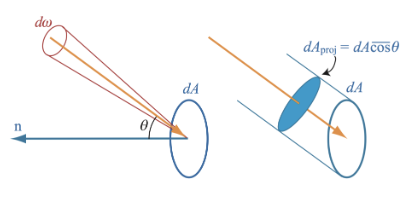
\includegraphics[scale=0.5]{figures/辐照亮度示意图.png}
    \caption{辐射亮度表示的是
    某个点在某个方向上的亮
    度,在计算机图形学中它是
    一束光的亮度,是渲染方程
    最终要计算的量}
\end{figure}

设$P(\xi,\eta)$是$A$面上的一个点,以面上任意一组方面的曲线为参考坐标系,现在在$P$点
取一面元$dA$,并围绕极角$(\alpha,\beta)$方向去一立体角$d\omega$,另外设$d\omega$方向与$dA$法线夹角为$\theta$,
则单位时间内由面元$dA$发射到$d\omega$的能量值$d\phi$可以表示为
\begin{equation}
    d\phi=L\overline{cos}\theta\ dA\ d\theta
\end{equation}

其中$L=L(\xi,\eta;\alpha,\beta)$是一个因子。

辐射亮度测试的是单束光的度量,它也正是感应器(例如人的眼睛,或者
场景中的虚拟摄像机)测量的度量,所以它在光照计算中特别重要。计算渲染
方程的目标就是计算出表面上的点到摄像机所在方向上的辐射亮度。另外值得
注意的是,L 的值不随距离发射点距离的变化而变化。

通常用两种不同的方式把$d\phi$分解成两个量的乘积,以表示它对$d\omega$和$d A$的显式关系
\begin{equation}
    d\phi=dId\omega=dEdA
\end{equation}

在接下来的两小节将分别讲述这两个新的度量 $I$和$E$。

\subsection*{辐照强度$I$}

辐射强度是指光源在特定方向上发射的光功率,单位立体角上的辐射能量。它描述了光源在某个方向上的辐射能力。
可以理解成从光源发出来通过某个面元的“光线的数量”的多少。

\begin{equation}
    I(\omega)=\equiv \frac{d\phi}{d\omega}
\end{equation}

\begin{figure}[H]
    \centering
    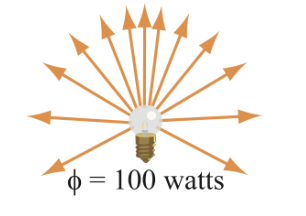
\includegraphics[scale=0.5]{figures/灯泡}
    \caption{一个灯泡在不同的
    方向上可能具有不同的辐射
    强度,辐射强度也是计算机\\
    图形学中表示各种光源光照
    的度量}
\end{figure}

比较辐射光照可以发现

\begin{equation}
    dI=\frac{d\phi}{d\omega}=L\ \overline{cos}\theta\ dA
\end{equation}

对一个面$A$积分得到
\begin{equation}
    I(\alpha,\beta)=\int L\ \overline{cos}\theta\ dA
\end{equation}

其中$I$称为面积$A$在方向$(\alpha,\beta)$辐照强度,其单位为$W/sr$,$I$是与距离无关的量,
但是他是与发射面积有关的,由于光源通常有一定的形状和面积,所以图形学通常使用$I$来表示一个光源的
辐射强度分布。

\subsection*{辐射照度}

定义:每一个面积上定义的能量

\begin{equation}
    dE=\frac{d\phi}{dA}=L\ \overline{cos}\theta\ d\omega
\end{equation}

对某个立体角积分有
\begin{equation}
    E(\xi,\eta)=\int L\ \overline{cos}\theta\ d\omega
\end{equation}

称为点 $(\xi ,\eta)$ 的辐射照度(irradiance),其单位为 $W /m^2$,它是点 $(\xi, \eta)$
沿各个方向对辐射亮度 L 的积分,值得注意的是,前面提到过,
在辐射度量学中,基本上考虑的是从面的一部分射出或者接收能量,所以辐射
照度虽然表述的是面上一个点的度量,但它实际上是通过该点所在的单位面积
来测量的,因为辐射亮度 L 也是通过单位面积来测量的。

\begin{figure}[H]
    \centering
    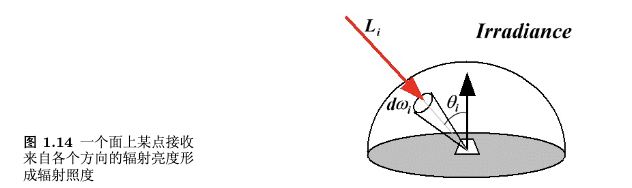
\includegraphics[scale=0.4]{figures/辐射照度模型.png}
    \caption{一个面上某点接收来自各\\个方向的辐射亮度形成辐射照度}
\end{figure}

回顾在布林冯模型中提到的Lamber's Cosine Law
\begin{equation}
    E=\frac{\phi}{A}cos\theta
\end{equation}

\begin{figure}[H]
    \centering
    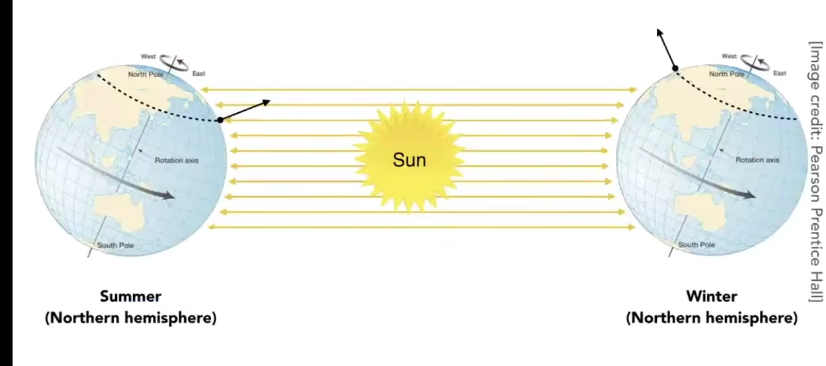
\includegraphics[scale=0.4]{figures/为什么有季节.png}
    \caption{为什么地球上有季节?}
\end{figure}

\subsection*{辐射度量学基本方程}

设$dA$是$P$处的面元,$QP=r$,又设$\theta$是$QP$与$dA$的法线夹角,则光源在单位时间内射过$dA$的能量是
$Id\omega$,其中$I$是光源沿$QP$方向的辐射强度,$d\omega$是$Q$所张立体角,如下图

\begin{figure}[H]
    \centering
    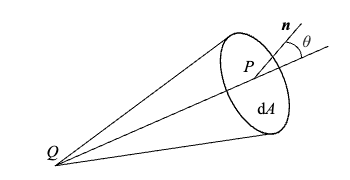
\includegraphics[scale=0.5]{figures/点光源所产生辐射照度.png}
    \caption{点光源所产生辐射照度}
\end{figure}

由基础几何学
\begin{equation}
    cos\theta\ dA\ == r^2d\omega
\end{equation}

根据$d\phi=dId\omega=dEdA$,所以有
\begin{equation}
    E=\frac{Icos\theta}{r^2}
\end{equation}

上式即辐射度量学的基本方程,他表达了所谓的照度余弦定理以及平方反比定律。

\section{Bidrectional Reflectance Distribution Function(BRDF)}

双向反射分布函数说明不同反射方向上分布的能量。试图理解反射到底是什么?

\subsection*{Reflecton at a Point}
\begin{figure}[H]
    \centering
    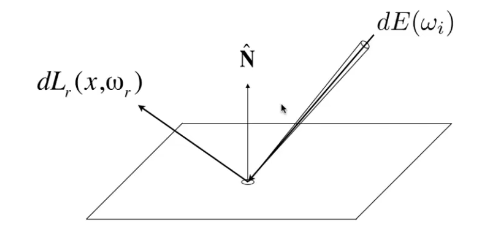
\includegraphics[scale=0.5]{figures/反射点.png}
    \caption{Reflecton at a Point}
\end{figure}

反射有两部分:

BRDF会如何被分配到不同的立体角上?

\begin{define}
    (BRDF)
    \begin{equation}
        f_r(\omega_i\rightarrow \omega_r)=\frac{dL_r(\omega_r)}{dE_i(\omega_i)}
    \end{equation}

\end{define}

\subsection*{The Reflection Equation}
\begin{figure}[H]
    \centering
    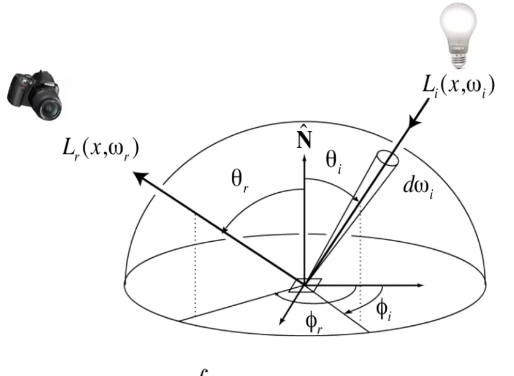
\includegraphics[scale=0.5]{figures/反射方程.png}
    \caption{Reflecton at a Point}
\end{figure}

\begin{equation}
    L_r(p,\omega_r)=\int_{H^2}f_r(p,\omega_i\rightarrow \omega_r)L_i(p,\omega_i)cos\theta_id\omega_i
\end{equation}

\subsection*{Challenge:Recursive Equation}

任何出射的radiance都有可能成为任何点入射点radiance。

\subsection*{The Rendering Equations}
\begin{equation}
    L_r(p,\omega_r)=\int_{H^2}f_r(p,\omega_i\rightarrow \omega_r)L_i(p,\omega_i)cos\theta_id\omega_i
\end{equation}

增加一个发射项使得其变得广义

\begin{framed}
    \begin{equation}
        L_o(p,\omega_o)=L_e(p,\omega_o)+\int_{\Omega_+}L_{i}(p,\omega_i)f_r(p,\omega_i,\omega_o)(n\cdot \omega_i)d\omega_i
    \end{equation}
\end{framed}

渲染方程可以让光线弹射多次。

\subsection*{渲染方程积分形式}

\subsection*{Linear Operator equation}

渲染方程算子形式。

\begin{equation}
    l(u)=e(u)+\int l(v)K(u,v)dv
\end{equation}

\begin{equation}
    L=E+KL
\end{equation}

\begin{figure}[H]
    \centering
    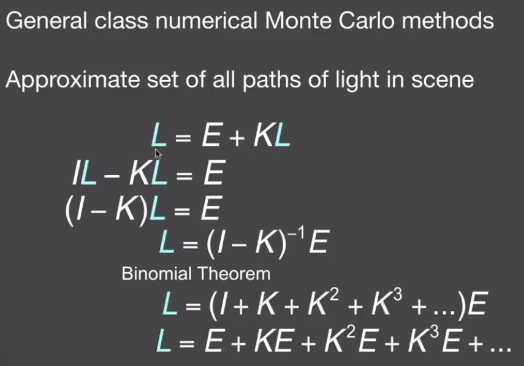
\includegraphics[scale=0.5]{figures/Rendering.png}
    \caption{Ray Tracing and Extensions}
\end{figure}

可以把能量分解成经过弹射次数的分解

\begin{equation}
    L=E+KE+K^2E+\cdots
\end{equation}

\begin{figure}[H]
    \centering
    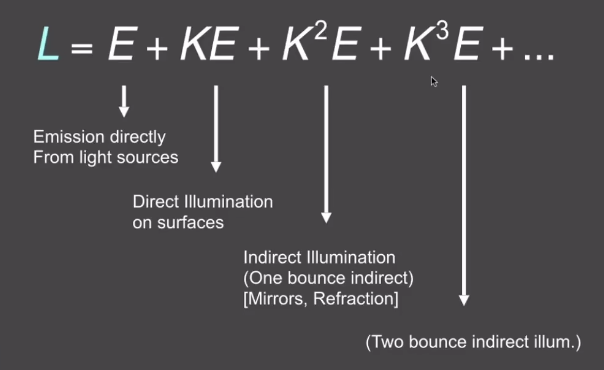
\includegraphics[scale=0.5]{figures/弹射次数的分解.png}
    \caption{弹射次数的分解}
\end{figure}

\section{Monte Carlo Integeration}

为什么需要蒙特卡洛积分?他是为了解决一个定积分
\begin{equation}
    \int_{a}^{b}f(x)dx
\end{equation}

相对于黎曼积分,蒙特卡洛积分是基于一种随机的采样的方法。

定积分服从随机分布
\begin{equation}
    X_i\sim p(x)
\end{equation}

则蒙特卡洛积分
\begin{equation}
    \int f(x)dx=\frac{1}{N}\sum\limits_{i=1}^{N}\frac{f(X_i)}{p(X_i)}
\end{equation}

\subsection*{Example:Uniform Monte Carlo Estimator}

\begin{equation}
    X_i\sim p(x)\equiv\frac{1}{b-a}
\end{equation}

\begin{equation}
    F_N=\frac{b-a}{N}\sum\limits_{i=1}^{N}f(X_i)
\end{equation}

\section{Path Tracing}

\subsection*{Motivation:Whitted-Style Ray Tracing}
Whitted Style的问题在于
\begin{enumerate}[itemindent=2em]
    \item 无法解决Glossy reflection;仍然认为沿着镜面反射是不对的;
    \item 漫反射物体
\end{enumerate}

\subsection*{怎么解决Whitted-Style Ray Tracing的问题}

渲染方程是基于物理的,所以绝对正确,采用蒙特卡洛方法解决渲染方程

\begin{equation}
    L_o(p,\omega_o)=\int_{\Omega_+}L_i(p,\omega_i)f_r(p,\omega_i,\omega_o)(n\cdot \omega_i)d\omega_i
\end{equation}

结论得到
\begin{equation}
    L_o(p,\omega_o)\approx \frac{1}{N}\sum\limits_{i=1}^{N}\frac{L_i(p,\omega_i)f_r(p,\omega_i,\omega_o)(n\cdot \omega_i)}{p(\omega_i)}
\end{equation}

\subsection*{Introducing Global illumination}
\begin{figure}[H]
    \centering
    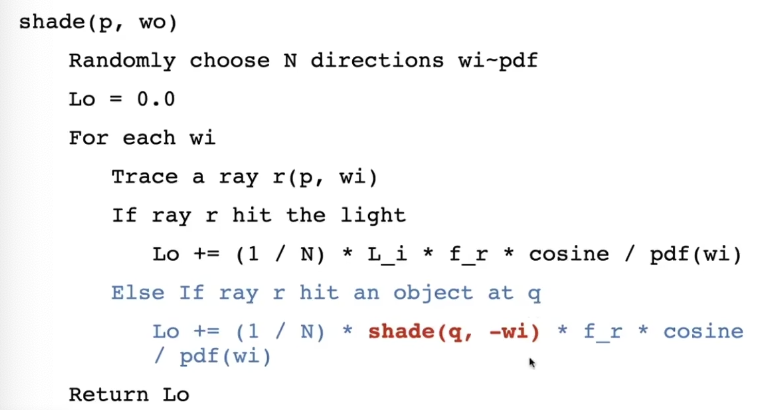
\includegraphics[scale=0.5]{figures/全剧光照.png}
    \caption{全局光照算法}
\end{figure}

以这种方式来做的问题,Problem1: 开销巨大
    \begin{figure}[H]
        \centering
        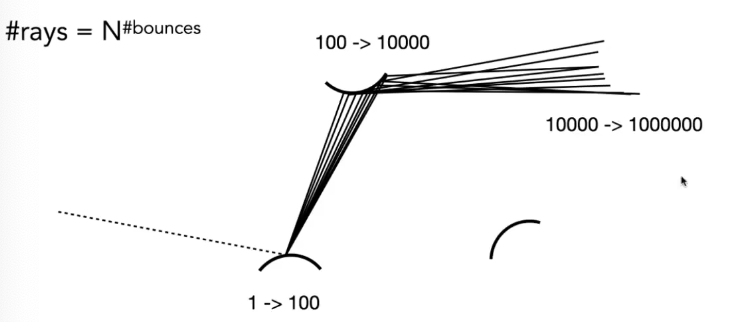
\includegraphics[scale=0.5]{figures/路径追踪开销巨大.png}
        \caption{路径追踪开销巨大}
    \end{figure}

    用$N=1$来做蒙特卡洛就是\textsl{路径追踪}

\textsl{Ray Generation}.

Problem2: 算法怎么停止?

\textsl{俄罗斯轮盘法}:以一定的概率停止往下走

\section{Sampling the Light}

浪费现象

\subsection*{pure math}

把渲染方程写成对于光源上的一个对积分的面积。

\begin{equation}
    d\omega=\frac{dA\ cos\theta'}{\Vert x'-x\Vert}
\end{equation}

则渲染方程可以写成
\begin{equation}
    L_o(x,\omega_o)=\int_AL_i(x,\omega_i)f_r(x,\omega_i,\omega_o)\frac{cos\theta\ cos\theta'}{\Vert x'-x\Vert}dA
\end{equation}

\section{Some Side Notes}